	\begin{frame}
		\Huge{\centerline{2APL platform}}
	\end{frame}
	
	\begin{frame}
		\frametitle{Requirements}
		\begin{itemize}
			\item OS: Windows, Mac OS X, Linux and Unix (Solaris);
			\item Java Runtime Environment (JRE) 6 or Java Developers Kit (JDK) 6;
			\item 2APL website URL: http://apapl.sourceforge.net/
		\end{itemize}
		
		\begin{figure}
			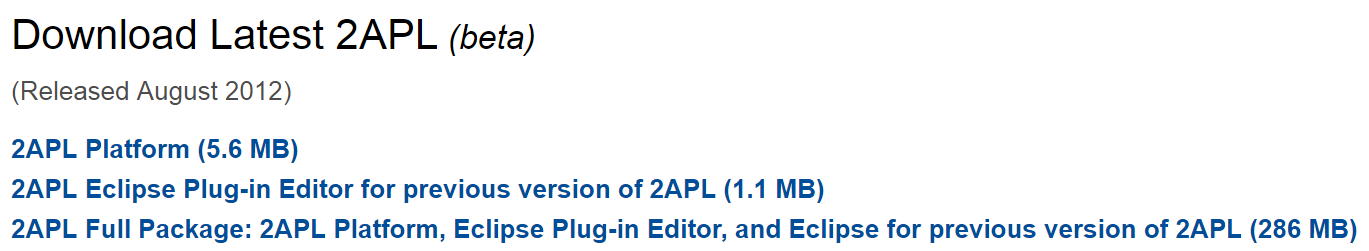
\includegraphics[width=0.9\linewidth]{images/2APLdownload.png}
			\caption{Download options for the platform on the 2APL website}
		\end{figure}
	\end{frame}
	
	
	\begin{frame}
		\frametitle{How to run the platform}
		2apl.jar can be run in two ways:
		\begin{itemize}
			\item directly (from the command line or windows interface);
			\item as a module for Eclipse;
		\end{itemize}
		
		The platform allows communication among agents and can run on several machines connected in a network (on top of the Jade platform);
		
		\begin{figure}
			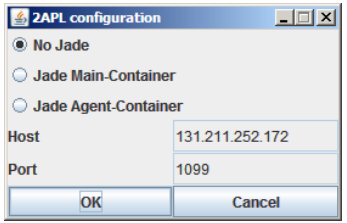
\includegraphics[width=0.4\linewidth]{images/2APLconf.png}
			\caption{2APL configuration options}
		\end{figure}
		
	\end{frame}
	
	\begin{frame}
		\frametitle{2APL project components}
		\begin{itemize}
			\item  The MAS specification file. This is a text file with the extension .mas that contains an XML specification of the multiagent system. The name and path to the source of all agents and environments that start in the application are denoted here.
			\item A 2APL agent file. This is a text file with the extension .2apl and contains the 2APL code of the agent.
			\item An environment file. This is a runnable JAR (with the extension .jar)
		\end{itemize}
	\end{frame}
	
	
	\begin{frame}
		\frametitle{2APL Platform}
		
		\begin{figure}
			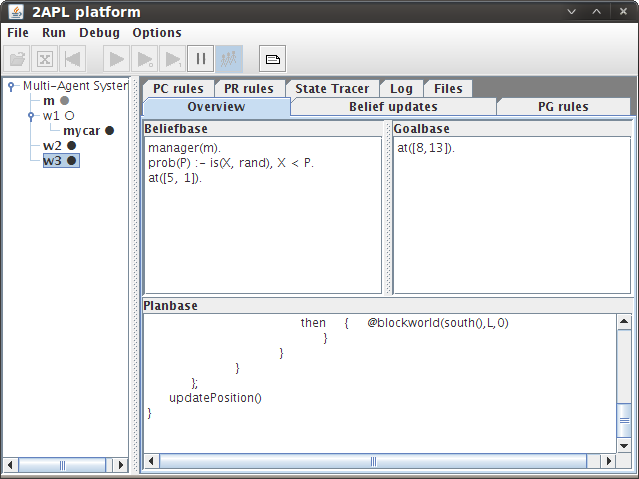
\includegraphics[width=0.75\linewidth]{images/2APLplatform.png}
			\caption{2APL platform interface}
		\end{figure}
		
	\end{frame}
	
	\begin{frame}
		\frametitle{Eclipse plug-in}
		\begin{figure}
			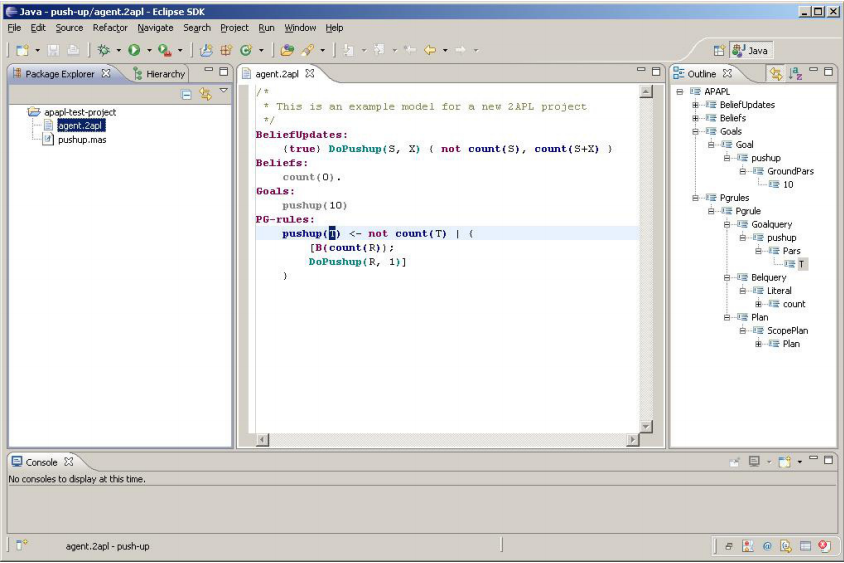
\includegraphics[width=0.85\linewidth]{images/2APLeclipse.png}
			\caption{2APL platform in Eclipse}
		\end{figure}
	\end{frame}
	
	
	\begin{frame}
		\frametitle{Additional Tools}
		\begin{block}{Monitoring Tools}
			\begin{itemize}
				\item Auto-update Overview tool;
				\item The State Tracer;
				\item Log tool.
			\end{itemize} 
		\end{block}
		
		These tools can be deactivated to improve the execution performance of the 2APL platform. The activation of the tools generates specific information and presents them in the corresponding tabs. 
		
	\end{frame}
	
	\begin{frame}
		\frametitle{Auto-update Overview tool}
		When this tab is active, the beliefs, goals, and plans of the current state of the selected agent are presented in the Beliefbase, Goalbase, and Planbase panels, respectively.
		
		\begin{figure}
			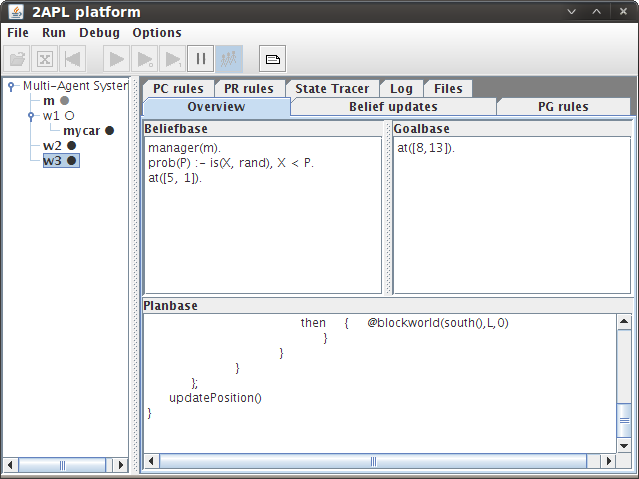
\includegraphics[width=0.65\linewidth]{images/2APLplatform.png}
		\end{figure}
	\end{frame}
	
	\begin{frame}
		\frametitle{State Tracer}
		Stores the beliefs, goals, and plans of all agents during execution. This tool allows a user to execute a multi-agent program for a while, pause the execution, and browse through the execution of each agent.
		
		\begin{figure}
			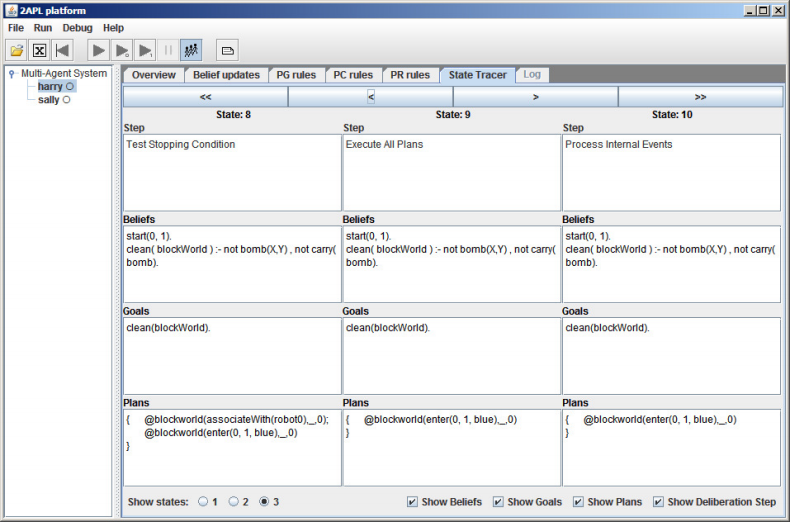
\includegraphics[width=0.65\linewidth]{images/2APLStateTracer.png}
		\end{figure}
	\end{frame}
	
	\begin{frame}
		\frametitle{Log tool}
		Presents information about the deliberation steps of individual agents. The user can browse through this window to see which deliberation steps have been preformed.
		
		\begin{figure}
			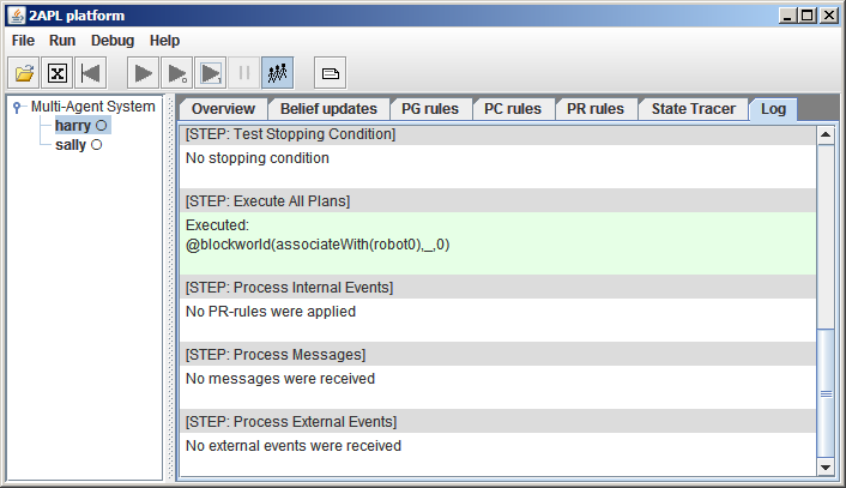
\includegraphics[width=0.65\linewidth]{images/2APLLog.png}
		\end{figure}
	\end{frame}
	
	\begin{frame}
		\frametitle{Summary of platform features}
		Programming Constructs
		\begin{itemize}
			\item \textbf{Multi-Agent System} Which and how many agents to create? Which environments? Which agent can access which environment?
			\item \textbf{Individual Agent} Beliefs, Goals, Plans, Events, Messages.
		\end{itemize}
		
		Programming Principles and Techniques
		\begin{itemize}
			\item \textbf{Abstraction} Procedures and Recursion in Plans;
			\item \textbf{Error Handling} Plan Failure and their revision by Internal Events, Execution of Critical Region of Plans;
			\item \textbf{Legacy Systems} Environment and External Actions;
			\item \textbf{Encapsulation} Including 2APL files in other 2APL files;
			\item \textbf{Autonomy} Adjustable Deliberation Process.
		\end{itemize}
		
	\end{frame}